% Options for packages loaded elsewhere
\PassOptionsToPackage{unicode}{hyperref}
\PassOptionsToPackage{hyphens}{url}
\documentclass[12pt, ]{article}

\usepackage{colortbl}
\usepackage{mathtools}
\usepackage{amsmath}
\usepackage{amsthm}
\usepackage{amssymb}
\usepackage[italicdiff]{physics}
\mathtoolsset{showonlyrefs}

% SPACING AND FONTS %%%%%%%%%%%%%%%%%%%%%%%%%%%%%%%%%%%%%%%%%%%%%%%%%%%%%%%%%%%%
\usepackage{iftex}
% CAREFUL: the order of font includes here is very important!
\ifPDFTeX
  \usepackage[OT1,T1]{fontenc}
  \usepackage[utf8]{inputenc}
  \usepackage{textcomp} % provide euro and other symbols
    \usepackage[p,osf,swashQ]{cochineal}
  \usepackage[cochineal,vvarbb]{newtxmath}
      \usepackage[scale=0.95]{biolinum}
    \usepackage[scale=0.95,varl]{inconsolata}
\else % if luatex or xetex
  \usepackage[scale=0.95,varl]{inconsolata}
  \usepackage{newpxtext}
  \usepackage{mathpazo}
    \usepackage[scale=0.95]{biolinum}
  \fi
\ifLuaTeX
  \usepackage{selnolig}  % disable illegal ligatures
\fi
\IfFileExists{microtype.sty}{% use microtype if available
  \usepackage[]{microtype}
  \UseMicrotypeSet[protrusion]{basicmath} % disable protrusion for tt fonts
}{}

\setlength{\parindent}{0pt}
\setlength{\parskip}{10pt plus 2pt minus 2pt}
\setlength{\emergencystretch}{3em} % prevent overfull lines
\widowpenalty=10000
\clubpenalty=10000
\flushbottom
\allowdisplaybreaks
\sloppy


% CORE PACKAGES %%%%%%%%%%%%%%%%%%%%%%%%%%%%%%%%%%%%%%%%%%%%%%%%%%%%%%%%%%%%
\usepackage[dvipsnames,svgnames,x11names]{xcolor}
\usepackage[lmargin=1.5in,rmargin=1.5in,tmargin=1.2in,bmargin=1.2in]{geometry}
\usepackage[format=plain,
  labelfont={bf,sf,small,singlespacing},
  textfont={sf,small,singlespacing},
  justification=justified,
  margin=0.25in]{caption}

% SECTIONS AND HEADINGS %%%%%%%%%%%%%%%%%%%%%%%%%%%%%%%%%%%%%%%%%%%%%%%%%%%%%%%%
\setcounter{secnumdepth}{4}
\usepackage{sectsty}
\usepackage[compact]{titlesec}
% short title
\makeatletter
\newcommand\@shorttitle{}
\newcommand\shorttitle[1]{\renewcommand\@shorttitle{#1}}
\usepackage{fancyhdr}
\fancyhf{}
\pagestyle{fancy}
\renewcommand{\headrulewidth}{0pt}
\fancyheadoffset{0pt}
%\lhead{\scshape \@shorttitle}
%\rhead{\scshape\today}
\cfoot{\thepage}
\makeatother
% abstract styling
\renewenvironment{abstract}{
  \centerline
  {\large\sffamily\bfseries Abstract}\vspace{-1em}
  \begin{quote}\small
}{
  \end{quote}
}

% PANDOC INCLUDES %%%%%%%%%%%%%%%%%%%%%%%%%%%%%%%%%%%%%%%%%%%%%%%%%%%%%%%%%%%%%%

\providecommand{\tightlist}{%
  \setlength{\itemsep}{0pt}\setlength{\parskip}{0pt}}\usepackage{longtable,booktabs,array}
\usepackage{calc} % for calculating minipage widths
% Correct order of tables after \paragraph or \subparagraph
\usepackage{etoolbox}
\makeatletter
\patchcmd\longtable{\par}{\if@noskipsec\mbox{}\fi\par}{}{}
\makeatother
% Allow footnotes in longtable head/foot
\IfFileExists{footnotehyper.sty}{\usepackage{footnotehyper}}{\usepackage{footnote}}
\makesavenoteenv{longtable}
\usepackage{graphicx}
\makeatletter
\def\maxwidth{\ifdim\Gin@nat@width>\linewidth\linewidth\else\Gin@nat@width\fi}
\def\maxheight{\ifdim\Gin@nat@height>\textheight\textheight\else\Gin@nat@height\fi}
\makeatother
% Scale images if necessary, so that they will not overflow the page
% margins by default, and it is still possible to overwrite the defaults
% using explicit options in \includegraphics[width, height, ...]{}
\setkeys{Gin}{width=\maxwidth,height=\maxheight,keepaspectratio}
% Set default figure placement to htbp
\makeatletter
\def\fps@figure{htbp}
\makeatother
% END PANDOC %%%%%%%%%%%%%%%%%%%%%%%%%%%%%%%%%%%%%%%%%%%%%%%%%%%%%%%%%%%%%%%%%%%

% USER INCLUDES %%%%%%%%%%%%%%%%%%%%%%%%%%%%%%%%%%%%%%%%%%%%%%%%%%%%%%%%%%%%%%%%
% additional LaTeX code for the "preamble" goes here
\makeatletter
\makeatother
\makeatletter
\makeatother
\makeatletter
\@ifpackageloaded{caption}{}{\usepackage{caption}}
\AtBeginDocument{%
\ifdefined\contentsname
  \renewcommand*\contentsname{Table of contents}
\else
  \newcommand\contentsname{Table of contents}
\fi
\ifdefined\listfigurename
  \renewcommand*\listfigurename{List of Figures}
\else
  \newcommand\listfigurename{List of Figures}
\fi
\ifdefined\listtablename
  \renewcommand*\listtablename{List of Tables}
\else
  \newcommand\listtablename{List of Tables}
\fi
\ifdefined\figurename
  \renewcommand*\figurename{Figure}
\else
  \newcommand\figurename{Figure}
\fi
\ifdefined\tablename
  \renewcommand*\tablename{Table}
\else
  \newcommand\tablename{Table}
\fi
}
\@ifpackageloaded{float}{}{\usepackage{float}}
\floatstyle{ruled}
\@ifundefined{c@chapter}{\newfloat{codelisting}{h}{lop}}{\newfloat{codelisting}{h}{lop}[chapter]}
\floatname{codelisting}{Listing}
\newcommand*\listoflistings{\listof{codelisting}{List of Listings}}
\makeatother
\makeatletter
\@ifpackageloaded{caption}{}{\usepackage{caption}}
\@ifpackageloaded{subcaption}{}{\usepackage{subcaption}}
\makeatother
\makeatletter
\@ifpackageloaded{tcolorbox}{}{\usepackage[skins,breakable]{tcolorbox}}
\makeatother
\makeatletter
\@ifundefined{shadecolor}{\definecolor{shadecolor}{rgb}{.97, .97, .97}}
\makeatother
\makeatletter
\makeatother
\makeatletter
\makeatother
% END USER INCLUDES %%%%%%%%%%%%%%%%%%%%%%%%%%%%%%%%%%%%%%%%%%%%%%%%%%%%%%%%%%%%

% BIBLIOGRAPHY %%%%%%%%%%%%%%%%%%%%%%%%%%%%%%%%%%%%%%%%%%%%%%%%%%%%%%%%%%%%%%%%%
\usepackage[]{natbib}
\bibliographystyle{apalike}

% Give it this name so that it works with ::: #refs
\newenvironment{CSLReferences}[2]{
\bibliography{bibliography.bib}
\clearpage
}{}

% LINKS %%%%%%%%%%%%%%%%%%%%%%%%%%%%%%%%%%%%%%%%%%%%%%%%%%%%%%%%%%%%%%%%%%%%%%%%
\usepackage{hyperref}
\usepackage{url}
\hypersetup{
  pdftitle={Locked Down, Voices Amplified: Nationalist Discourse in the Era of COVID-19},
  pdfauthor={Joyce Wang},
  colorlinks=true,
  linkcolor={black},
  filecolor={Maroon},
  citecolor={VioletRed4},
  urlcolor={DodgerBlue4},
  pdfcreator={LaTeX via pandoc}}

% TITLE, AUTHOR, DATE %%%%%%%%%%%%%%%%%%%%%%%%%%%%%%%%%%%%%%%%%%%%%%%%%%%%%%%%%%
\title{\sffamily\bfseries\huge\parfillskip=0pt
\rightskip=0pt plus .5\textwidth
\leftskip=0pt plus .5\textwidth
\emergencystretch=.3\textwidth Locked Down, Voices Amplified:
Nationalist Discourse in the Era of COVID-19}
\shorttitle{Locked Down, Voices Amplified: Nationalist Discourse in the Era of COVID-19}
\author{\textbf{Joyce Wang}
 }
\date{}


\begin{document}
\allsectionsfont{\sffamily}

\maketitle

\begin{abstract}
This study examines the impact of state policy on cyber-nationalism, focusing on the reaction of China's online nationalist group, 'Little Pink,' to Shanghai's COVID-19 lockdown. Using an original dataset of social media posts from Weibo, I employ a difference-in-difference approach to analyze changes in nationalist sentiment before and after the implementation of the lockdown. The findings reveal a complex temporal pattern: an initial decrease in nationalist expressions immediately after the announcement of lockdown, followed by a significant increase within two weeks. This suggests an adaptive response among online nationalists, where initial dissatisfaction gives way to heightened nationalist discourse, potentially as a counter to negative perceptions of state policies. The study highlights the complex relationship between state actions and cyber-nationalism and contribute to our understanding of the dynamics of online political discourse in authoritarian regimes. The Github repository is \url{https://github.com/joycewang071/AQRD-Dec-2023} 

\end{abstract}

\ifdefined\Shaded\renewenvironment{Shaded}{\begin{tcolorbox}[enhanced, interior hidden, borderline west={3pt}{0pt}{shadecolor}, breakable, sharp corners, boxrule=0pt, frame hidden]}{\end{tcolorbox}}\fi



% USER BODY %%%%%%%%%%%%%%%%%%%%%%%%%%%%%%%%%%%%%%%%%%%%%%%%%%%%%%%%%%%%%%%%%%%%

\hypertarget{introduction}{%
\section{Introduction}\label{introduction}}

COVID-19 heightened economic and political uncertainty and has become a transformative moment for nationalism in China \citep{woods2020covid}. China's adoption and initial success of its Zero-Covid policy showcased its ability to handle crises and satisfy the national pride of Chinese nationalists, especially when compared with the rapidly increasing COVID-19 death rate in the US, which they perceive as a failure of the US in controlling the pandemic \citep{wang2021crisis,woods2020covid}. In this context, Chinese people are likely to become more nationalistic, observing China's effectiveness and efficiency in controlling the case numbers and death rate of COVID-19 \citep{woods2020covid}. However, there's also a potential for decreased nationalism due to the significant disruption of personal life caused by the party-state’s strict implementation of the Zero-COVID policy \citep{wang2021crisis}.  

Among China's various policies, lockdowns are considered the strictest. Since the first wave of COVID, there have been several lockdowns, including Hubei’s from January to March 2020, Shanghai’s from March 28 to June 1, 2022, and Chengdu’s in September 2022, among others. Shanghai's Lockdown, with its large affected population and extended duration, particularly caught our attention. 

The online group I aim to focus on is Little Pink, China’s online nationalists. The term "Little Pink" originated from a pink-colored discussion forum focused on "Boy's Love," but later evolved to describe active young online nationalists after members of Little Pink participated in the "cross-strait memes war" protesting Taiwan's pro-independence political activities\citep{fang2018demystifying}.

This paper examines the impact of Shanghai's Lockdown on cyber-nationalism, with a focus on Little Pink in Shanghai during COVID-19. Moreover, by conducting a difference-in-difference experiment on Shanghai's Little Pink, this study investigates the causality of how personally experiencing the Lockdown influenced public opinion, particularly among those who already exhibited nationalistic preferences. The results show that Shanghai’s lockdown initially decreased Little Pink’s nationalism when the policy was first announced, but the implementation of the lockdown in the subsequent two weeks led to an increase in their online nationalist sentiments.


\hypertarget{data}{%
\section{Data}\label{data}}

To study cyber-nationalism, I collected an original dataset of posts from China’s social media platform Weibo, which serves as a proxy for Twitter in China. The data is subject to post-censorship, as the collection timestamp is 12 months later than the data generation time \citep{king2013censorship}.

Since Little Pinks are defined as active online nationalists, I identified them based on their active and positive interactions with nationalistic influencers on Weibo. I initially selected 19 nationalistic influencers on Weibo, based on news reports and netizen consensus \footnote{``"state-backed" Online abuse: How did the online version of the Cultural Revolution come about? '' 2022. \emph{WHYNOT}.
  \url{https://www.wainao.me/wainao-reads/state-backed-online-abuse-04132022}.}. From February to August 2022, I chose the first 7 to 10 posts from these influencers' monthly posting history. From each post, I selected the 7 to 10 most popular comments, typically receiving the most "likes" from other users. The authors of these comments are the Little Pink subjects of this investigation.

Considering that Shanghai’s lockdown spanned from March 28 to June 1, 2022, I collected posts from February 1 to June 1 to compare pre- and post-lockdown cyber-nationalism. For each Little Pink, I retrieved their IP location from their posts in May. According to a Weibo announcement on April 28, 2022, Weibo began revealing the IP address of each comment, indicating the user's real provincial location, which became publicly available in May \footnote{``Announcement of IP Location upgrade'' 2022. \emph{Sina Visitor System}.  \url{https://weibo.com/1934183965/LqvYeCdBu}.}. I filtered for users who were active and consistently posting from the same provincial location in May. In addition, I collected their self-identified gender, whether they are Weibo-verified active users and their number of fans from their profile pages. The dataset includes 416,320 posts from 11,233 Little Pink, with 863 users having an IP location in Shanghai.

For each post, I applied a pre-trained Fasttext classifier to assign each post a continuous nationalistic score ranging from 0 to 1. The training dataset for Fasttext contained 3,281 positive samples and 6,562 negative samples from Weibo. I then set a threshold of 0.3 to label posts with scores higher than 0.3 as nationalistic (1), and those with lower scores as non-nationalistic (0).

Since the study involves analyzing provincial differences in public sentiments, an important factor is the provincial Covid case number. I used data from the news platform NetEase News, which has collected COVID-related health data from the National Health Commission and local health departments at all levels. From its website, I compiled the daily confirmed, healed, and deceased case numbers for every province in China from February 1 to June 1, 2022. I summed the daily COVID case statistics into weekly intervals, including 31 provinces. 

\begin{figure}[]

{\centering \includegraphics[width=1\textwidth,height=\textheight]{figures/Covid_number.png}}
\caption{\label{fig-covid}Trend of Case Numbers between Shanghai (black) and Non-Shanghai (grey) Provinces with lockdown division (red)}

\end{figure}

Figure~\ref{fig-covid} compares the trend of case numbers between Shanghai and non-Shanghai provinces. It shows that Shanghai’s lockdown began in an early stage of virus spread. During the time of Shanghai’s lockdown, the city had considerably higher numbers than the sum of the remaining provinces in all three aspects of COVID-19 cases. This indicates that no other province experienced a COVID outbreak at a similar level of severity and intensity in terms of virus spread and public attention during Shanghai’s lockdown.





Furthermore, I aggregated post-level sentiments into user levels at weekly intervals. Table~\ref{descriptive} shows the summary statistics. On average, Little Pink published 4.81 nationalistic posts from February 1 to June 1, accounting for 13\% of their posting history. User-level statistics show that only 30\% of Little Pink are female and 3\% are verified users. Being a Weibo-verified user requires a certain level of activity and authentication \footnote{``How to apply for identity verification''  \emph{Sina Visitor System}.  \url{https://kefu.weibo.com/faqdetail?id=37}.}.. The low proportion of verified users suggests that most try to remain anonymous. The gender disparity implies a bias in nationalistic discussions.

\begin{table}
\caption{\textbf{Summary Statistics}}
\label{descriptive}
\input{tables/descriptive.tex}
\end{table}



\hypertarget{method}{%
\section{Method}\label{method}}

This project adopts the difference-in-difference (DID) method to test the impact of Shanghai's lockdown on Shanghai's Little Pinks. The model I use is:

\[ T_{it} = \alpha + \beta_{1}D_{i,t} + \beta_{2}D_{i,t - 1} + \beta_{3}D_{i,t - 2} + \gamma X_{i,t} + \eta_{i} + \theta_{t} + \epsilon_{it}, \]

where \( i \) indexes each province and \( t \) indexes the time period, week. \( T_{it} \) is the nationalism level of Little Pink for province \( i \) in week \( t \). I operationalize users’ nationalism level by the number of nationalistic posts they publish and the proportion of nationalist posts among all posts per week.

\( D_{it} \) is a dummy treatment indicator, which indicates whether the user is currently under Shanghai’s lockdown. Specifically, the treatment equals one when the user’s IP location is Shanghai, and the time is between March 28 and June 1 in 2022.

\( D_{i, t-1} \) and \( D_{i, t-2} \) are the lagged treatment indicators from the last week and two weeks ago. We consider two weeks’ lagged treatment because the quarantine time for COVID is two weeks. \( X_{i,t} \) is a vector of control variables at the user and province level. User-level covariates include gender, Weibo-verification status, and fan numbers, as the expression of nationalism might be influenced by gender norms, anonymity, and users’ online impact. I also include provincial COVID case numbers, as people might adjust their attitudes towards the party-state based on its performance in controlling COVID, reflected by the fluctuation of COVID case numbers. Additionally, I standardize the fan numbers and case numbers when running the model, so that the scale of variables can be more comparable. \( \alpha \), \( \beta \) and \( \gamma \) are parameters to be estimated. \( \eta_{i} \) are province fixed effects parameters also to be estimated, \( \theta_{t} \) are week fixed effects parameters, and \( \epsilon_{it} \) is the error term.

We adopt ordinary least squares (OLS) models and report province-clustered standard errors to account for within-province correlations in our data. The primary hypotheses evaluated in this article are that lockdown and lagged lockdown effects cause a decrease in nationalism level (\( \beta_{1} \), \( \beta_{2} \), \( \beta_{3} < 0 \)).

Next, I discuss the conditions and assumptions for Difference-in-Difference models to work.

I first checked the user-level covariate balance in Table~\ref{covariate_balance}. Covariate balance is the degree to which the distribution of covariates is similar across levels of the treatment. After running t-tests for gender, verification, and fan numbers on the treatment variable in the pretreatment dataset, I found that the p-values for all three tests were larger than 0.05. Therefore, we cannot reject the null hypothesis, suggesting that we do not have sufficient evidence to claim that the users in the pretreatment dataset are different. In other words, we can assume that the Little Pink in Shanghai and non-Shanghai provinces were similar before Shanghai’s lockdown.
 
\begin{table}
\caption{\textbf{Covariate Balance}}
\label{covariate_balance}
\input{tables/covariate_balance.tex}
\end{table}

Secondly, I drew event study plots of lead and lag lockdown effects on two measurements of outcome variables: the number and proportion of nationalistic posts. Event study plots are used to evaluate the treatment effects of the pre- and post-treatment periods. The result is shown in Figure~\ref{fig-event} The formula for the event study is as follows: 
\[ T_{it} = \alpha + \beta_{1}D_{i,t} + \beta_{2}D_{i,t - 1} + \beta_{3}D_{i,t - 2} + \beta_{4}D_{i,t - 3} +\beta_{5}D_{i,t +1}+ \beta_{6}D_{i,t + 2}+\beta_{7}D_{i,t + 3} + \eta_{i} + \theta_{t} + \epsilon_{it}, \]

 When week < 0, the lead lockdown effects (\( \beta_{5} \), \( \beta_{6} \), \( \beta_{7} \)) should be insignificant if the nationalism levels of Shanghai and Non-Shanghai follow a parallel trend before the lockdown. From the plots, we can generally see that only the 2-week lead lockdown effect is insignificant, which might imply that the parallel trend assumption for Difference-in-Difference might not always hold and we need more nuanced observations of when it will work. Also, \( \beta_{1} \) is consistently significantly negative, and \( \beta_{2} \) and \( \beta_{3} \) are significantly positive, suggesting that lockdown has an instantaneous negative effect and a two-week lagged positive effect on Little Pink’s nationalism level. Moreover, the negative \( \beta_{4} \) also means that after three weeks, the lockdown effects become negative again in a statistically significant way.

\begin{figure}[]

{\centering 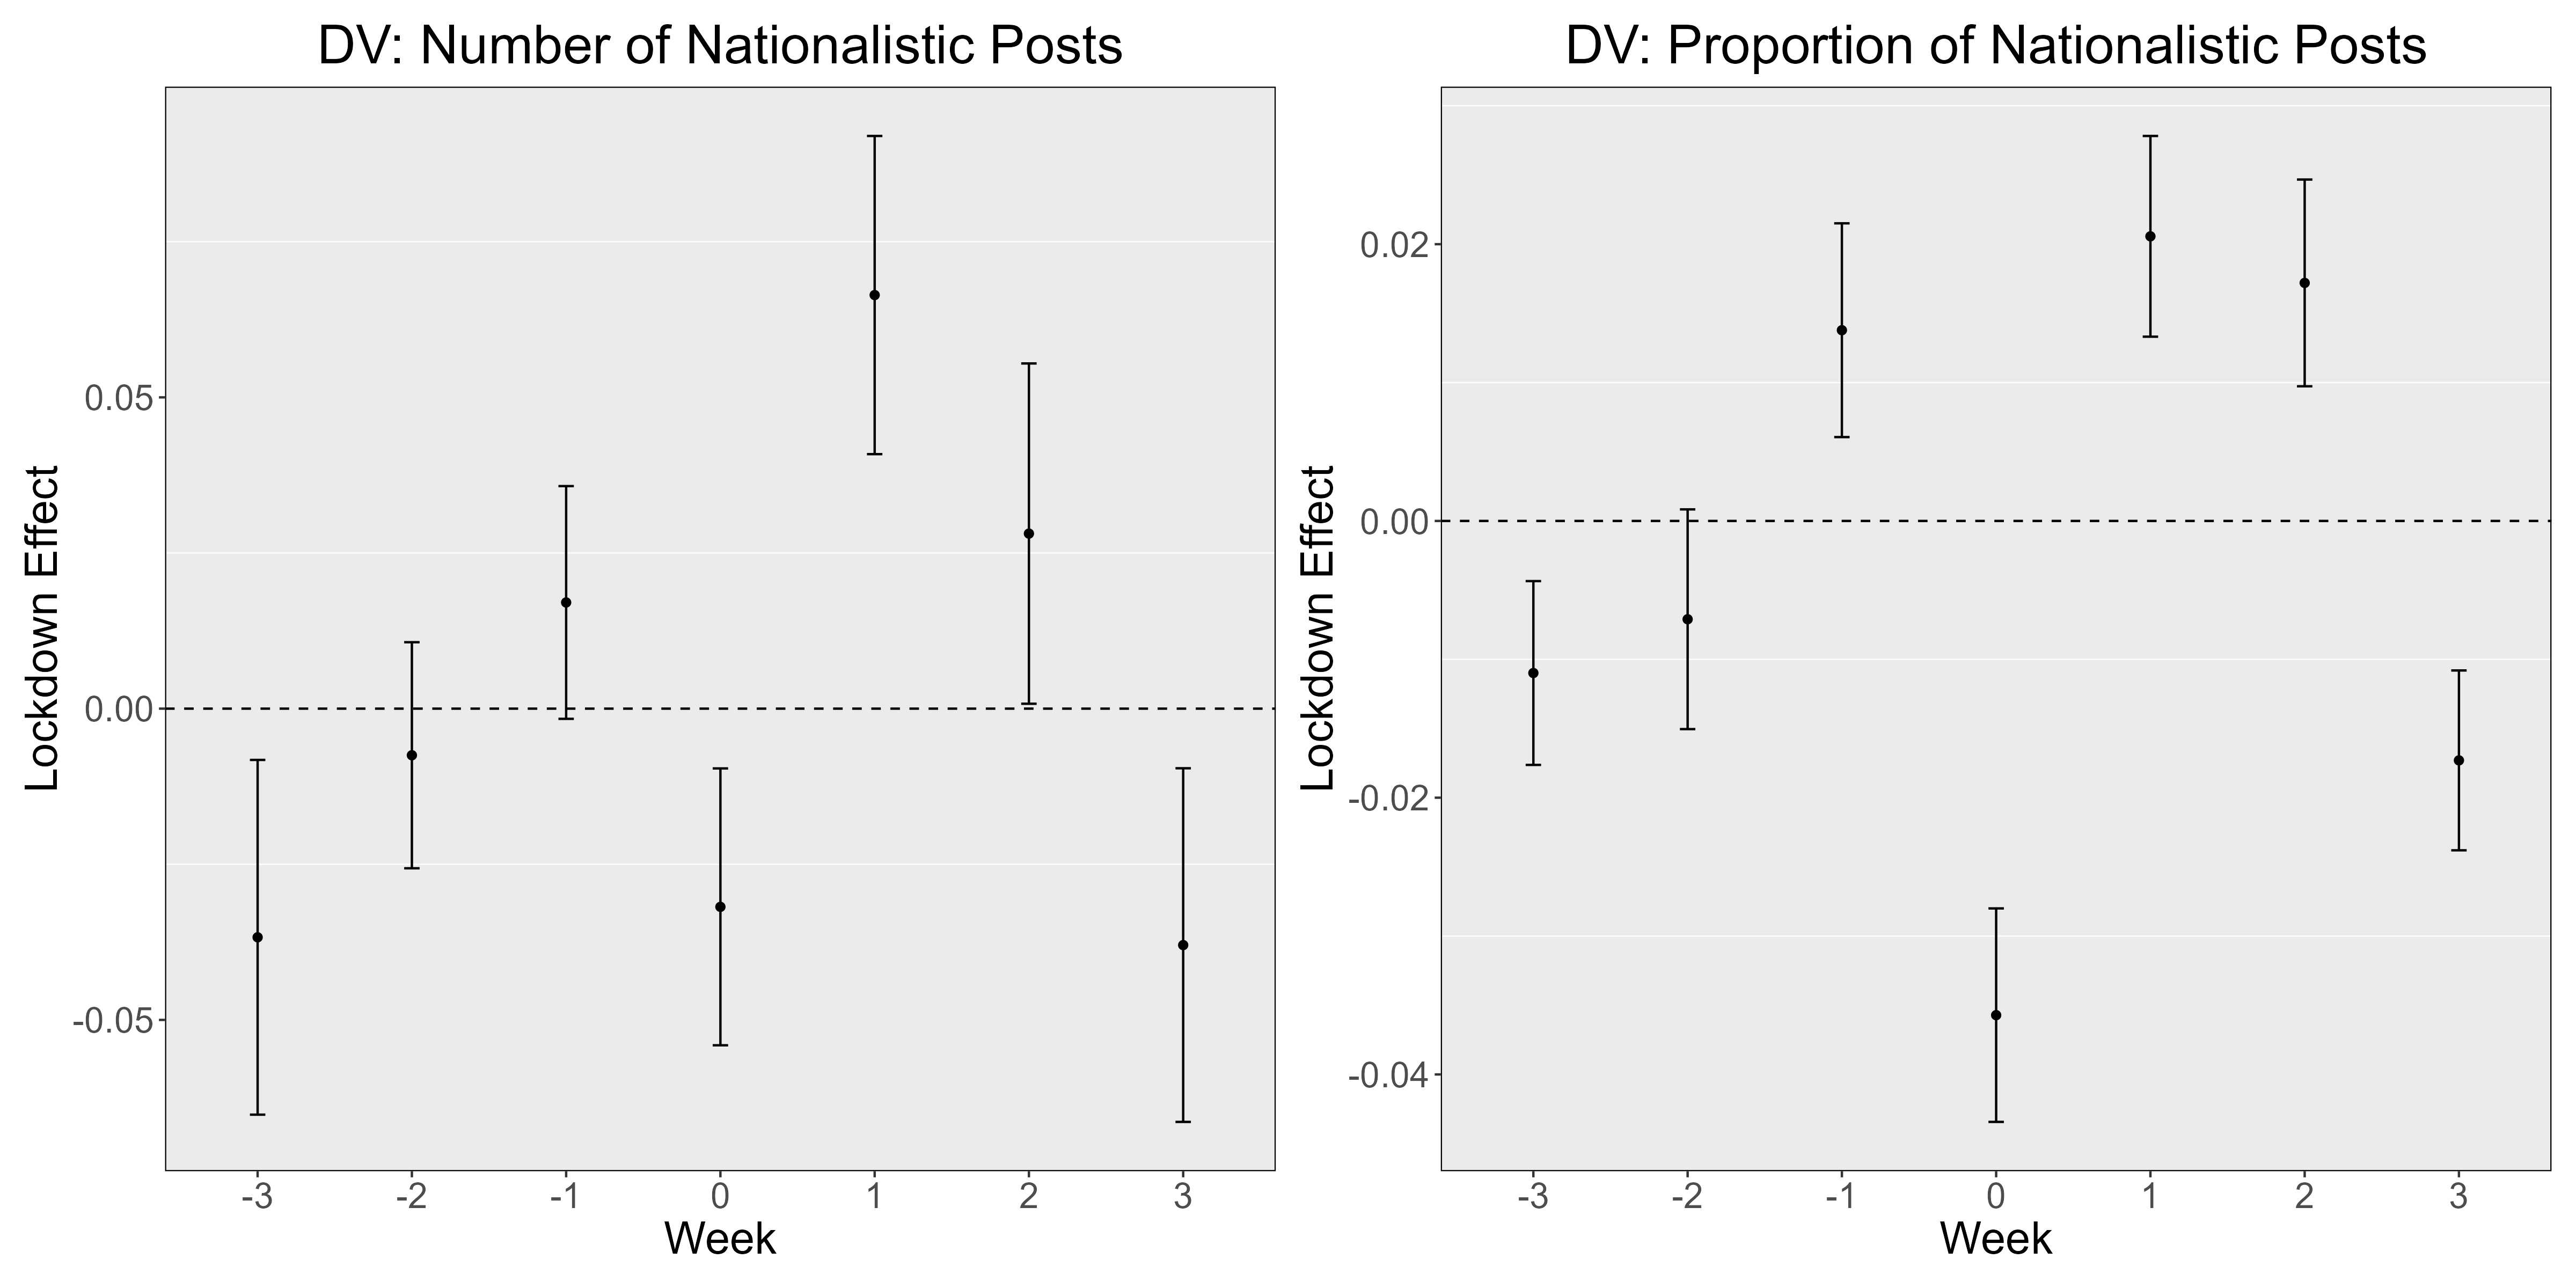
\includegraphics[width=1\textwidth,height=\textheight]{figures/Event_study.png}}
\caption{\label{fig-event}Event Study Plot}

\end{figure}



\hypertarget{results}{%
\section{Results}\label{results}}

Figure~\ref{fig-trend} compares the Shanghai and Non-Shanghai Little Pinks’ nationalism levels before and after Shanghai’s lockdown. March 28, the first day of Week 13, marks the beginning of Shanghai’s lockdown. Weeks 6 to 12 constitute the pre-lockdown period and weeks 13-22 fall within the duration of Shanghai’s lockdown. 

\begin{figure}[]

{\centering 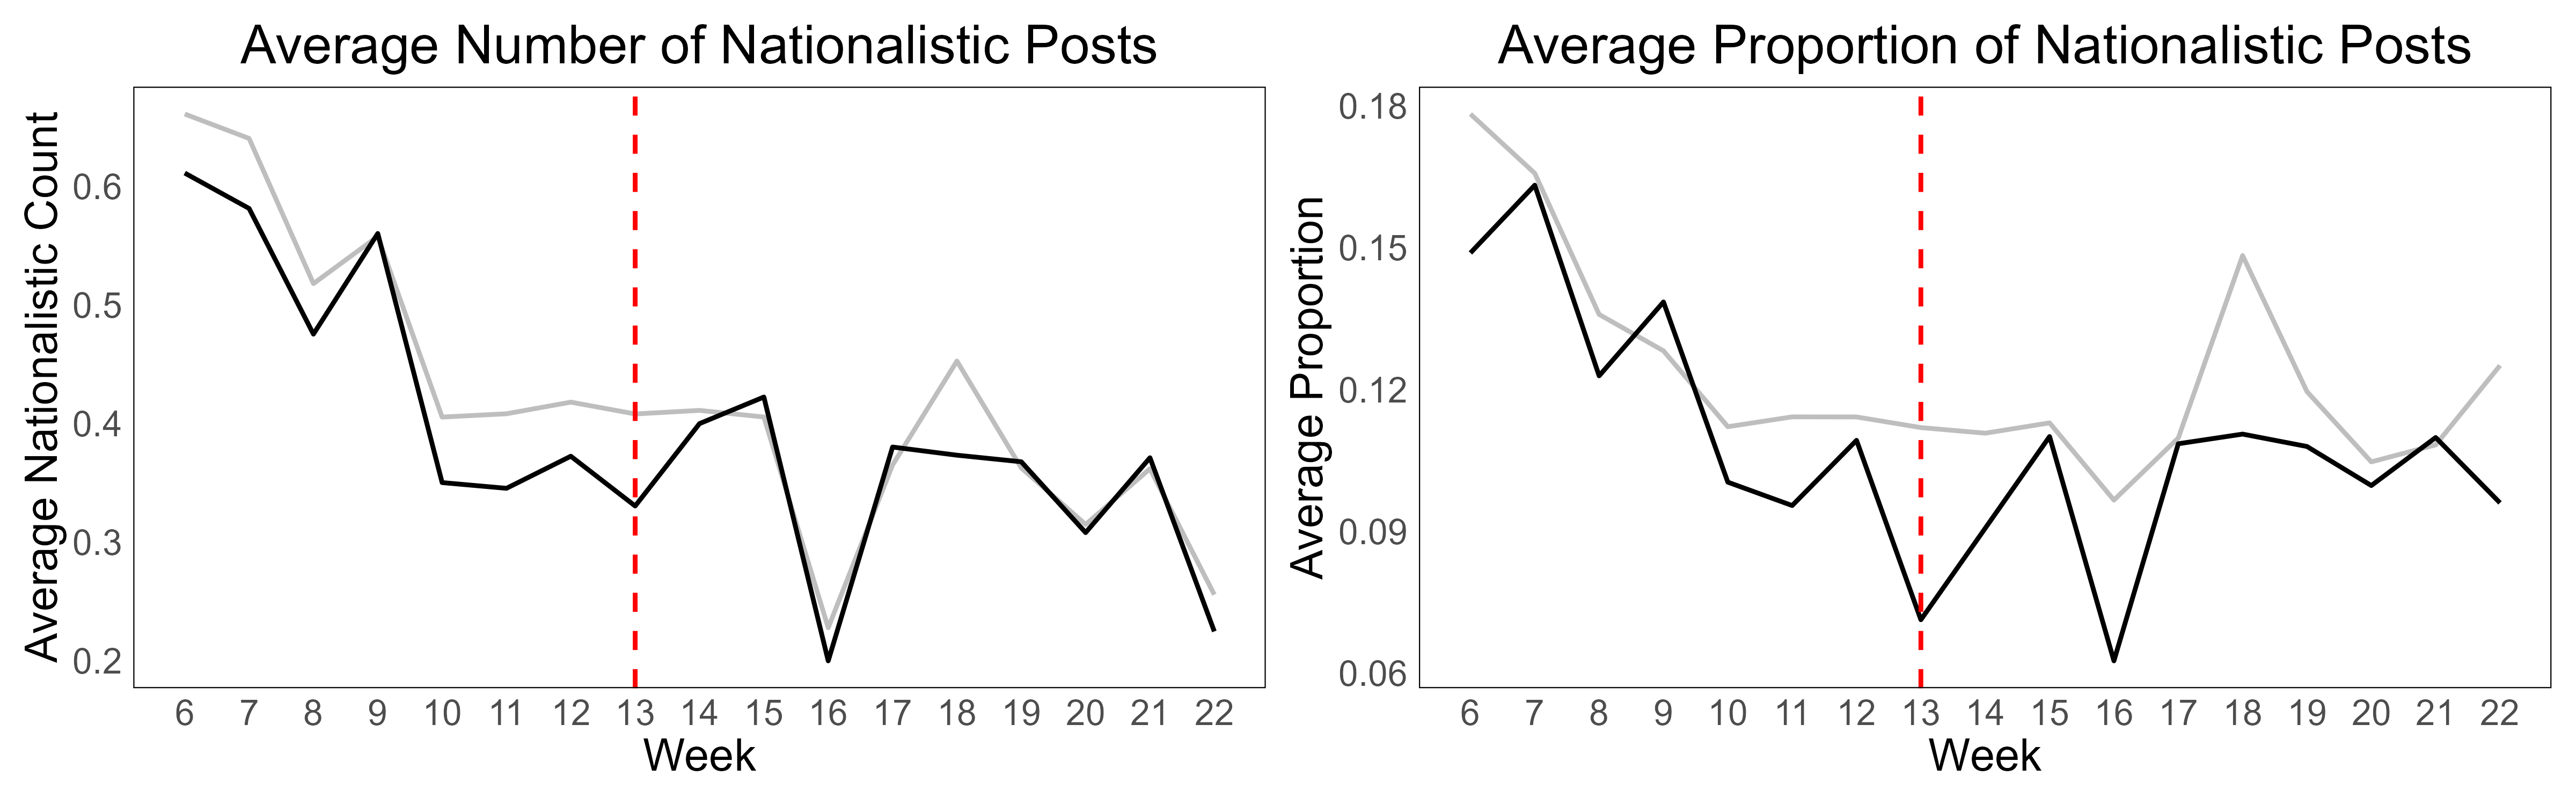
\includegraphics[width=1\textwidth,height=\textheight]{figures/trend.png}}
\caption{\label{fig-trend} Trend of Nationalism Level between Shanghai(black) and Non-Shanghai(grey) Provinces with lockdown division (red) }

\end{figure}

The weekly average number of nationalistic posts ranges from 0.2 to 0.8. Temporally, the lockdown leads Little Pink to post less as time progresses. Moreover, compared with Non-Shanghai Little Pink, Shanghai Little Pink generally posted less in the pre-lockdown period, except for week 9. However, one week after the start of the lockdown, Shanghai users began posting more, reaching a level similar to that of non-Shanghai users. The weekly average proportion of nationalistic posts ranges from 6\% to 18\%. Before week 10, the performances of Shanghai and non-Shanghai users were very similar. However, starting from week 10, Shanghai users began to post a smaller proportion of nationalistic content compared with Non-Shanghai Little Pink.

The above analysis shows that, compared with non-Shanghai users, even if the absolute number of nationalistic posts increases, the proportion of nationalism decreases in Shanghai users’ online expressions.

\begin{table}[htbp]
\caption{\textbf{Regression Table}}
\label{regression}
\input{tables/regression.tex}
\end{table}


Table~\ref{regression} presents a regression table with the main findings across step-wise specifications, and all models control for province and week-fixed effects.



I will first discuss the cases where the nationalism level is measured by the absolute number of nationalistic posts. Without any control variables, the lockdown has a positive effect on nationalism. However, after controlling for the lagged lockdown treatments, the effect of the lockdown ranges from -0.034 to -0.042, with small standard errors. This indicates that Shanghai’s lockdown reduces the weekly number of nationalistic posts by around 0.035. Moreover, the one-week lagged lockdown effect has been consistently positive and statistically significant, ranging from 0.058 to 0.066, which means that the lockdown from the previous week tends to increase the number of nationalist posts by 0.066. Additionally, being female and being a verified user on Weibo are associated with lower levels of nationalism, while the weekly confirmed and deceased COVID case numbers positively influence the nationalism level of Little Pink.

The results are generally similar when measuring the nationalism level by the proportion of nationalistic posts. Shanghai’s lockdown has a significant negative effect on Little Pink’s nationalism level in that week. Specifically, the lockdown reduces the proportion of nationalistic posts by around 3.5 percentage points. However, the one-week and two-week lagged lockdown effects increase the nationalism level by 2 percentage points. A possible explanation is that Little Pink in Shanghai initially felt dissatisfied with the party-state’s policy when the lockdown was implemented. However, as time went by, they adapted to the new lifestyle. Simultaneously, due to the increasing negative sentiments about the lockdown policy and the party-state in general, Little Pinks felt compelled to counter these opinions by overstating nationalistic views, akin to their actions during the "cross-strait memes war" to protest Taiwan's pro-independence political activities and assert China’s policies. This over-compensating narrative may also explain why an increase in weekly confirmed and deceased COVID cases accelerates their nationalistic sentiments, while an increase in COVID cases should have proved the failure of policies and decrease their satisfaction and nationalism.


\hypertarget{conclusion}{%
\section{Conclusion}\label{conclusion}}

In conclusion, this project uses a difference-in-difference approach to analyze an original dataset of social media posts, with a specific focus on the impact of Shanghai's lockdown on the online nationalist group known as 'Little Pink' in China during the COVID-19 pandemic.  This study deepens our understanding of the dynamic interaction between state policy and cyber-nationalism. Our findings show that the immediate effect of the lockdown was a decrease in the expression of nationalist sentiments among Shanghai-based Little Pinks. However, this initial reaction was followed by an increase in nationalistic expressions over the subsequent one to two weeks. This pattern suggests that initial dissatisfaction with state policies may eventually lead to an overcompensated reaffirmation of nationalist sentiments, driven by Little Pinks’ desire to counter criticism of the state's handling of the pandemic.

Some limitations should be acknowledged. For example, fasttext might not be the best classifier for supervised learning on this dataset, given the complexity of nationalistic expressions in the Chinese context. Also, the covid case dataset has a small proportion of mislabeling, leading the case number to be below zero, which requires further verification on the data sources. Moreover, all models have a relatively low R-square, which means that the explaining power of models can be improved in future research. Despite this, this research contributes to our understanding of cyber-nationalism in authoritarian contexts, particularly in situations of crisis. It highlights the complex ways in which citizens' expressions of nationalism can be shaped by their experiences and perceptions of state policies.



\hypertarget{refs}{}

\begin{CSLReferences}{0}{0}\end{CSLReferences}




% END BODY %%%%%%%%%%%%%%%%%%%%%%%%%%%%%%%%%%%%%%%%%%%%%%%%%%%%%%%%%%%%%%%%%%%%%



\end{document}
